\documentclass[a4paper,11pt]{article}
\usepackage[
    a4paper,
    left=2cm,
    right=2cm,
    top=3cm,
    bottom=2.7cm
]{geometry}
\usepackage[T1]{fontenc}
\usepackage{times}
\usepackage[ruled,vlined,linesnumbered,longend]{algorithm2e} % Changed to algorithm2e
\usepackage{pdflscape}
\usepackage{caption}
\usepackage{lipsum}
\usepackage{circuitikz}
\usepackage{float}
\usepackage[utf8]{inputenc}
\usepackage[czech,shorthands=off]{babel}
\usepackage{csquotes} 
\usepackage{subcaption}
\usepackage{microtype}
\usepackage{booktabs, graphicx, setspace}
\usepackage{multirow}
\usepackage{amsmath} 
\usepackage{amssymb} 
\usepackage{amsthm}
\usepackage{hyperref}


\newtheorem{theorem}{Věta}
\newtheorem{definition}{Definice}

\begin{document}

\begin{titlepage}
    \begin{center}
        {\Huge\textsc{Vysoké učení technické v Brně}\\}
        \vspace{0.5em}
        {\huge \textsc{Fakulta informačních technologií}\\}
        \vfill
        \vspace{-5cm}
        {\huge Typografie a publikování – 3. projekt\\}
        \vspace{0.6em}
        {\huge \textbf{Tabulky a obrázky}}
        \vfill
        \Large{\today} \hfill \Large{Radim Pokorný (xpokorr00)}
    \end{center}
\end{titlepage}

\section{Úvodní strana}
    Název práce umístěte do zlatého řezu a nezapomeňte uvést dnešní (today) datum a vaše jméno a příjmení.
\section{Tabulky}
    Pro sázení tabulek můžeme použít buď prostředí \texttt{ tabbing } nebo prostředí \texttt{ tabular }.
\subsection{Prostředí \texttt{ tabbing }}
    Při použití \texttt{ tabbing } vypadá tabulka následovně:
    \begin{tabbing}
        
        \textbf{Ovoce} \hspace{2cm} \= \textbf{Množství} \hspace{1cm} \= \textbf{Jednotka} \hspace{1cm} \= \textbf{Cena za jedn.} \hspace{1cm} \= \textbf{Cena celková} \kill
        \textbf{Ovoce} \> \textbf{Množství} \> \textbf{Jednotka} \> \textbf{Cena za jedn.} \> \textbf{Cena celková} \\
        Jablka \> 3 \> kg \> 25{,}90 Kč \> 77{,}70 Kč \\
        Hrušky \> 2{,}5 \> kg \> 27{,}40 Kč \> 68{,}50 Kč \\
        Vodní melouny \> 1 \> kus \> 35{,--} Kč \> 35{,--} Kč \\
    \end{tabbing}
    Toto prostředí se dá také použít pro sázení algoritmů, ovšem hodnější je použít prostředí \texttt{ algorithm } nebo \texttt{ algorithm2e } (viz sekce 3).
\subsection{Prostředí \texttt{ tabular }}
    Další možnosti, jak vytvořit tabulku, je použít prostředí \texttt{ tabular }. Tabulky pak budou vypadat takto\footnote{Kdyby byl problém s \texttt{ cline}, zkuse se podívat třeba sem: http://www.abclinuxu.cz/tex/poradna/show/325037}:
    \begin{center}
        \begin{table}[h!]
            \centering
            \begin{tabular}{ |c|c|c| } 
            \hline
            & \multicolumn{2}{|c|}{\textbf{Cena}} \\ 
            \cline{2-3}
            \textbf{Měna} & \textbf{Nákup} & \textbf{Prodej} \\
            \hline
            EUR & 23,26 & 24,93 \\ 
            GBP & 29,56 & 29,83 \\ 
            USD & 22,27 & 23,12 \\ 
            \hline
            \end{tabular}
            \caption{Tabulka kurzů k aktuálnímu dni}
            \label{tab:kurzy}
        \end{table}
        \begin{table}[ht]
            \centering
            \begin{minipage}[t]{0.10\textwidth}
                \centering
                \begin{tabular}{|c|c|}
                \hline
                A & $\lnot A$ \\ 
                \hline
                \textbf{P} & N \\ 
                \hline
                \textbf{O} & O \\ 
                \hline
                \textbf{X} & X \\ 
                \hline
                \textbf{N} & P \\ 
                \hline
                \end{tabular}
                \label{tab:negace}
            \end{minipage}
            \hspace{0mm}
            \begin{minipage}[t]{0.25\textwidth}
                \centering
                \begin{tabular}{|c|c|c|c|c|c|}
                    \hline
                    \multicolumn{2}{|c|}{\multirow{2}{*}{$A \land B$}} & \multicolumn{4}{c|}{B} \\ 
                    \cline{3-6}
                    \multicolumn{2}{|c|}{} & \textbf{P} & \textbf{O} & \textbf{X} & \textbf{N} \\ 
                    \hline
                    \multirow{4}{*}{\textbf{A}} & \textbf{P} & P & O & X & N \\ 
                    \cline{2-6}
                    & \textbf{O} & O & O & N & N \\ 
                    \cline{2-6}
                    & \textbf{X} & X & N & X & N \\ 
                    \cline{2-6}
                    & \textbf{N} & N & N & N & N \\ 
                    \hline
                \end{tabular}
                \label{tab:implikace}
            \end{minipage}
            \hspace{0mm}
            \begin{minipage}[t]{0.25\textwidth}
                \centering
                \begin{tabular}{|c|c|c|c|c|c|}
                    \hline
                    \multicolumn{2}{|c|}{\multirow{2}{*}{$A \lor B$}} & \multicolumn{4}{c|}{B} \\ 
                    \cline{3-6}
                    \multicolumn{2}{|c|}{} & \textbf{P} & \textbf{O} & \textbf{X} & \textbf{N} \\ 
                    \hline
                    \multirow{4}{*}{\textbf{A}} & \textbf{P} & P & P & P & P \\ 
                    \cline{2-6}
                    & \textbf{O} & P & O & P & O \\ 
                    \cline{2-6}
                    & \textbf{X} & P & P & X & X \\ 
                    \cline{2-6}
                    & \textbf{N} & P & O & X & N \\ 
                    \hline
                \end{tabular}
                \label{tab:implikace}
            \end{minipage}
            \hspace{0mm}
            \begin{minipage}[t]{0.25\textwidth}
                \centering
                \begin{tabular}{|c|c|c|c|c|c|}
                    \hline
                    \multicolumn{2}{|c|}{\multirow{2}{*}{$A \to B$}} & \multicolumn{4}{c|}{B} \\ 
                    \cline{3-6}
                    \multicolumn{2}{|c|}{} & \textbf{P} & \textbf{O} & \textbf{X} & \textbf{N} \\ 
                    \hline
                    \multirow{4}{*}{\textbf{A}} & \textbf{P} & P & O & X & N \\ 
                    \cline{2-6}
                    & \textbf{O} & P & O & P & O \\ 
                    \cline{2-6}
                    & \textbf{X} & P & P & X & X \\ 
                    \cline{2-6}
                    & \textbf{N} & P & P & P & P \\ 
                    \hline
                \end{tabular}
                \label{tab:implikace}
            \end{minipage}
            \caption{Protože Kleeneho trojhodnotová logika už je ,,zastaralá'', uvádíme si zde příklad čtyřhodnotové logiky}
            \label{tab:quadtabule}
        \end{table}

    \end{center}
    \pagebreak
    \section{Algoritmy}
    Pokud budeme chtít vysázet algoritmus, můžeme použít prostředí \texttt{ algorithm }\footnote{http://ftp.cstug.cz/pub/tex/CTAN/macros/latex/contrib/algorithms/algorithms.pdf} nebo \texttt{ algorithm2e }\footnote{http://ftp.cstug.cz/pub/tex/CTAN/macros/latex/contrib/algorithm2e/doc/algorithm2e.pdf}.
    Příklad použití prostředí \texttt{ algorithm2e } viz Algoritmus 1.
    \IncMargin{1.5em}
    \begin{algorithm}
        \SetAlgoLined
        \DontPrintSemicolon
        \LinesNumbered
        \SetNlSty{}{}{}
        \SetAlgoNlRelativeSize{0}
        \caption{\textsc{FastSLAM}}
        \label{alg:cap}
        
        % KwIn and KwOut will now respect the 1.5em indentation
        \KwIn{$(X_{t-1}, u_t, z_t)$}
        \KwOut{$X_t$}
        \DecMargin{1.5em}
        $\overline{X_t} = X_t = 0$\;
        \SetAlgoNoLine
        \For{$k = 1$ \KwTo $M$}{
            $x_t^{[k]} = \text{sample\_motion\_model}(u_t, x_{t-1}^{[k]})$\;
            $\omega_t^{[k]} = \text{measurement\_model}(z_t, x_t^{[k]}, m_{t-1})$\;
            $m_t^{[k]} = \text{updated\_occupancy\_grid}(z_t, x_t^{[k]}, m_{t-1})$\;
            $X_t \gets X_t + \langle x_t^{[k]}, \omega_t^{[k]} \rangle$\;
        }
        \SetAlgoNoLine
        \For{$k = 1$ \KwTo $M$}{
            draw $i$ with probability $\approx \omega_t^{[i]}$\;
            add $\langle x_k^{[x]}, m_k^{[t]} \rangle$ to $X_t$\;
        }
        \Return{$X_t$}
    \end{algorithm}

    \section{Obrázky}
    Do našich článků můžeme samozřejmě vkládat obrázky. Pokud je obrázkem fotografie, můžeme
    klidně použít bitmapový soubor. Pokud by to ale být nějaké schéma nebo něco podobného, 
    je dobrým zvykem takovýto obrázek vytvořit vektorově.
    \begin{figure}[H]
        \centering
        \begin{subfigure}[b]{0.25\textwidth}
            \centering
            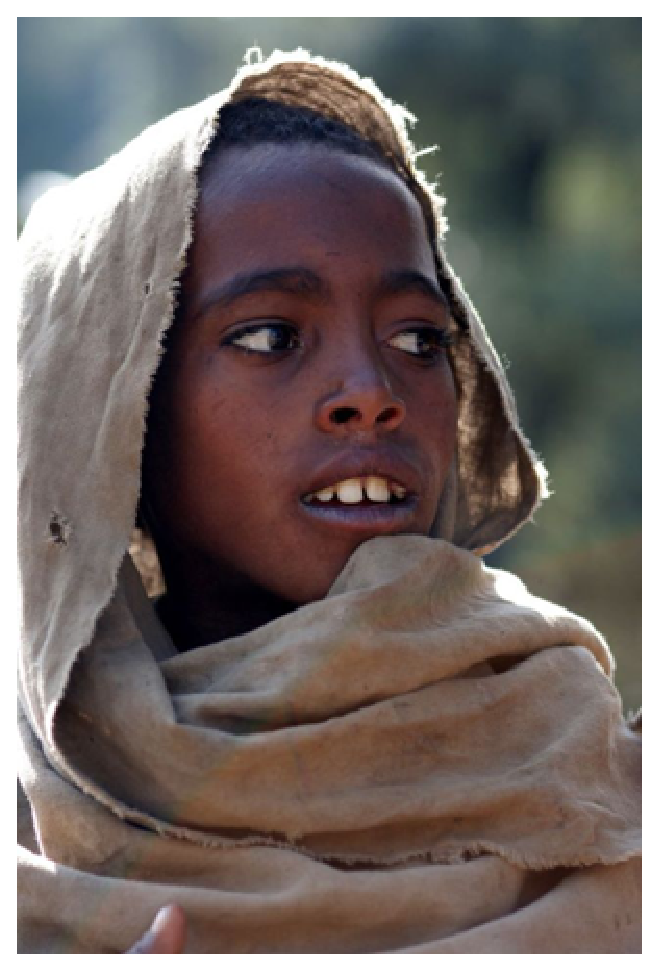
\includegraphics[width=\textwidth]{etiopan.eps}
        \end{subfigure}
        \begin{subfigure}[b]{0.25\textwidth}
            \centering
            \reflectbox{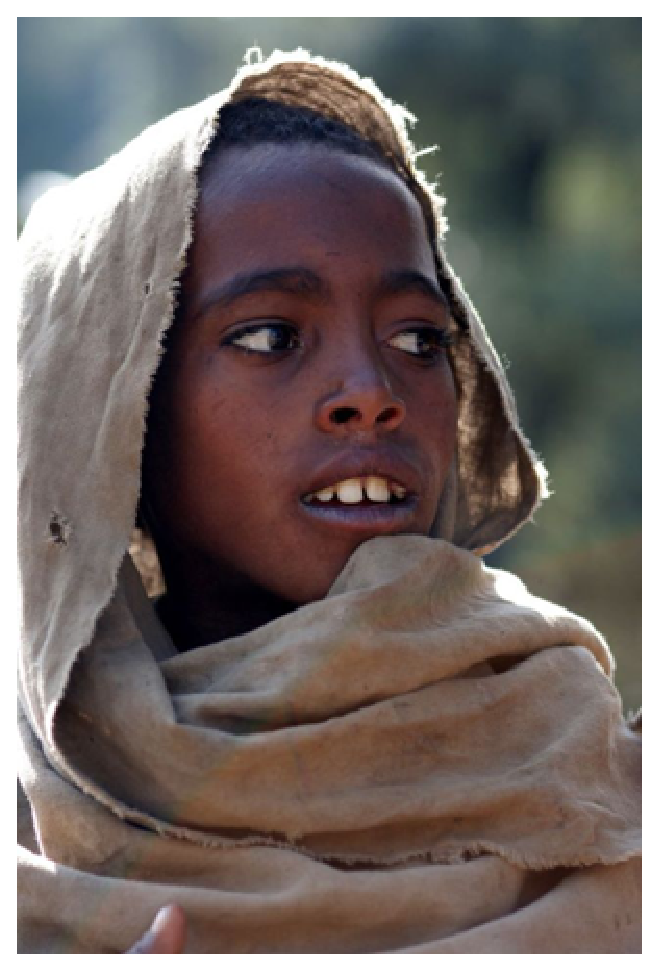
\includegraphics[width=\textwidth]{etiopan.eps}}
        \end{subfigure}
        \caption{Malý Etiopánek a jeho bratříček}
        \label{fig:etiopanecek}
    \end{figure}
    \pagebreak
    Rozdíl mezi vektorovým $\ldots$
        \begin{figure}[H]
            \centering
            
\includegraphics[width=0.45\textwidth]{oniisan.eps}
            \caption{Vektorový obrázek}
        \end{figure}
        $\ldots$ a bitmapovým obrázkem    
        \begin{figure}[H]
            \centering
            
\includegraphics[width=0.5\textwidth]{oniisan2.eps}
            \caption{Bitmapový obrázek}
            
        \end{figure}
        \noindent{se projeví například při zvětšení.}

        Odkazy (nejen ty) na obrázky 1,2 a 3, na tabulky 1 a 2 a také na algoritmus 1 jsou udělány pomocí křížových odkazů. Pak je ovšem potřeba zdrojový soubor přeložit dvakrát.
        
        Vektorové obrázky lze vytvořit i přímo v \LaTeX{u}, například pomocí prostředí \texttt{ picture }.

        \pagebreak
        \begin{landscape}
        \begin{figure}[!ht]
            \centering
            \resizebox{1\textwidth}{!}{%
            \begin{circuitikz}
            \tikzstyle{every node}=[font=\LARGE]
            \draw [short] (9,13.5) -- (9,8.25);
            \draw [short] (9,13.5) -- (20.75,13.5);
            \draw [short] (20.75,13.5) -- (20.75,8.25);
            \draw [short] (9,8.25) -- (20.75,8.25);
            \draw [short] (13.75,8.25) -- (13.75,11.5);
            \draw [short] (13.75,11.5) -- (15.5,11.5);
            \draw [short] (15.5,11.5) -- (15.5,8.25);
            \draw [short] (14,8.25) -- (14,11.25);
            \draw [short] (14,11.25) -- (14.5,11.25);
            \draw [short] (14.5,11.25) -- (14.5,8.25);
            \draw [short] (14,10.75) -- (14.5,10.75);
            \draw [short] (14,10.25) -- (14.5,10.25);
            \draw [short] (14,9.75) -- (14.5,9.75);
            \draw [short] (14,9.25) -- (14.5,9.25);
            \draw [short] (14,8.75) -- (14.5,8.75);
            \draw [short] (9,13.5) -- (14.75,15.25);
            \draw [short] (14.75,15.25) -- (20.75,13.5);
            \draw [short] (10,11.5) -- (10,10.25);
            \draw [short] (10,10.25) -- (12,10.25);
            \draw [short] (12,10.25) -- (12,11.5);
            \draw [short] (10,11.5) -- (12,11.5);
            \draw [short] (10.25,11.25) -- (10.25,10.5);
            \draw [short] (10.25,10.5) -- (11.75,10.5);
            \draw [short] (11.75,10.5) -- (11.75,11.25);
            \draw [short] (10.25,11.25) -- (11.75,11.25);
            \draw [short] (17,11.5) -- (17,10.25);
            \draw [short] (17,10.25) -- (19.25,10.25);
            \draw [short] (19.25,10.25) -- (19.25,11.5);
            \draw [short] (17,11.5) -- (19.25,11.5);
            \draw [short] (17.25,11.25) -- (17.25,10.5);
            \draw [short] (17.25,10.5) -- (19,10.5);
            \draw [short] (19,10.5) -- (19,11.25);
            \draw [short] (17.25,11.25) -- (19,11.25);
            \draw [short] (20.75,13.25) -- (26,13.25);
            \draw [short] (26,13.25) -- (26,12.75);
            \draw [short] (26,12.75) -- (20.75,12.75);
            \draw [short] (22,9.25) -- (22,9.75);
            \draw [short] (25,9.25) -- (25,9.75);
            \draw [short] (22,9.75) -- (22.25,10);
            \draw [short] (25,9.75) -- (24.75,10);
            \draw [short] (22.25,10) -- (22.5,10.5);
            \draw [short] (22.5,10.5) -- (23,10.75);
            \draw [short] (23,10.75) -- (24.25,10.75);
            \draw [short] (24.25,10.75) -- (24.5,10.5);
            \draw [short] (24.5,10.5) -- (24.75,10);
            \draw [short] (22,9.25) -- (22,9);
            \draw [short] (22,9) -- (25,9);
            \draw [short] (25,9.25) -- (25,9);
            \draw [short] (22,9) -- (22,8.5);
            \draw [short] (22,8.5) -- (22.5,8.5);
            \draw [short] (22.5,8.5) -- (22.5,9);
            \draw [short] (25,9) -- (25,8.5);
            \draw [short] (25,8.5) -- (24.5,8.5);
            \draw [short] (24.5,8.5) -- (24.5,9);
            \draw [short] (22.25,9.25) -- (23,9.25);
            \draw [short] (24.75,9.25) -- (24,9.25);
            \draw [short] (22.25,9.25) -- (22.25,9.5);
            \draw [short] (22.25,9.5) -- (22.75,9.5);
            \draw [short] (22.75,9.5) -- (23,9.25);
            \draw [short] (24,9.25) -- (24.25,9.5);
            \draw [short] (24.25,9.5) -- (24.75,9.5);
            \draw [short] (24.75,9.5) -- (24.75,9.25);
            \draw [short] (22.25,10) -- (24.75,10);
            \draw [short] (22.5,10) -- (22.75,10.5);
            \draw [short] (22.75,10.5) -- (24.25,10.5);
            \draw [short] (24.25,10.5) -- (24.5,10);
            \draw [short] (22.25,9.5) -- (22.5,10);
            \draw [short] (24.5,10) -- (24.75,9.5);
            \draw [short] (22.75,9.5) -- (24.25,9.5);
            \draw [short] (23,9.25) -- (24,9.25);
            \draw [short] (23,9.5) -- (23.25,9.25);
            \draw [short] (24,9.5) -- (23.75,9.25);
            \draw [short] (23.25,9.5) -- (23.5,9.25);
            \draw [short] (23.5,9.25) -- (23.75,9.5);
            \draw [short] (23,9.25) -- (23,9);
            \draw [short] (23.25,9.25) -- (23.25,9);
            \draw [short] (23.5,9.25) -- (23.5,9);
            \draw [short] (23.75,9.25) -- (23.75,9);
            \draw [short] (24,9.25) -- (24,9);
            \draw [short] (22.5,9) -- (22.75,8.75);
            \draw [short] (22.75,8.75) -- (24.25,8.75);
            \draw [short] (24.25,8.75) -- (24.5,9);
            \draw [short] (24,9) -- (23.75,8.75);
            \draw [short] (23.75,9) -- (23.5,8.75);
            \draw [short] (23.25,9) -- (23.5,8.75);
            \draw [short] (23,9) -- (23.25,8.75);
            \draw [short] (22.25,10.25) -- (22,10.25);
            \draw [short] (22,10.25) -- (22,10);
            \draw [short] (22,10) -- (22.25,10);
            \draw [short] (22.25,10.25) -- (22.25,10);
            \draw [short] (24.75,10) -- (24.75,10.25);
            \draw [short] (24.75,10.25) -- (25,10.25);
            \draw [short] (24.75,10) -- (25,10);
            \draw [short] (25,10.25) -- (25,10);
            \draw [short] (25.25,12.75) -- (25.25,8.25);
            \draw [short] (25.25,8.25) -- (25.5,8.25);
            \draw [short] (25.5,8.25) -- (25.5,12.75);
            \draw [short] (21.25,12.75) -- (21.25,8.25);
            \draw [short] (21.25,8.25) -- (23.25,8.25);
            \draw [short] (23.25,8.25) -- (25.25,8.25);
            \draw [short] (21.5,8.25) -- (21.5,12.5);
            \draw [short] (21.5,12.5) -- (21.5,12.75);
            \draw [short] (21.5,11.5) -- (25.25,11.5);
            \draw [short] (21.5,8.5) -- (22,9.25);
            \draw [short] (25.25,9.5) -- (25,9);
            \draw [short] (24.5,8.25) -- (24.75,8.5);
            \draw [short] (23.75,10) -- (23.75,10.25);
            \draw [short] (23.75,10.25) -- (24.25,10.25);
            \draw [short] (24.25,10.25) -- (24.25,10);
            \draw [short] (22.75,10) -- (22.75,10.25);
            \draw [short] (22.75,10.25) -- (23.25,10.25);
            \draw [short] (23.25,10.25) -- (23.25,10);
            \draw [short] (17.25,10.5) -- (19,11.25);
            \draw [short] (10.25,10.5) -- (11.75,11.25);
            \draw [short] (10,10.25) -- (9.75,10.25);
            \draw [short] (9.75,10.25) -- (9.75,10);
            \draw [short] (9.75,10) -- (12.25,10);
            \draw [short] (12,10.25) -- (12.25,10.25);
            \draw [short] (12.25,10.25) -- (12.25,10);
            \draw [short] (17,10.25) -- (16.75,10.25);
            \draw [short] (16.75,10.25) -- (16.75,10);
            \draw [short] (16.75,10) -- (19.5,10);
            \draw [short] (19.25,10.25) -- (19.5,10.25);
            \draw [short] (19.5,10.25) -- (19.5,10);
            \draw [short] (20,8.25) -- (20,13);
            \draw [short] (20.25,13) -- (20.25,8.25);
            \draw [short] (20.25,13) -- (20.75,13);
            \draw [short] (20,13) -- (9,13);
            \draw [short] (9,13.25) -- (20.75,13.25);
            \draw [short] (15.25,10) -- (15.25,9.75);
            \draw [short] (15.25,9.75) -- (15,9.75);
            \draw  (10,17) circle (0.5cm);
            \draw [short] (10,16.5) -- (10,16.25);
            \draw [short] (10,17.5) -- (10,17.75);
            \draw [short] (10.5,17) -- (10.75,17);
            \draw [short] (9.5,16.5) -- (9,16);
            \draw [short] (10.5,16.5) -- (11,16);
            \draw [short] (10.5,17.5) -- (10.75,17.75);
            \draw [short] (9.75,17.5) -- (9.5,18);
            \draw [short] (9.5,17) -- (8.5,17);
            \draw [short] (26,12.75) -- (25.5,12.25);
            \draw [short] (21.25,12.25) -- (20.75,12.25);
            \draw [short] (22,11.25) -- (21.75,11);
            \draw [short] (22,10.75) -- (21.75,10.5);
            \draw [short] (9,13.5) -- (8.5,13);
            \draw [short] (8.5,13) -- (8.5,8.25);
            \draw [short] (8.5,8.25) -- (9,8.25);
            \draw [short] (8.75,11.25) -- (8.5,11);
            \draw [short] (8.75,11.25) -- (8.75,10.25);
            \draw [short] (8.75,10.25) -- (8.5,10);
            \draw [short] (8.75,10.25) -- (8.75,10);
            \draw [short] (8.75,10) -- (8.5,9.75);
            \draw [short] (8.75,11.25) -- (8.5,10.5);
            \draw [short] (9,13) -- (8.5,12.5);
            \draw [short] (9,13.25) -- (8.5,12.75);
            \draw [short] (20.75,13) -- (26,13);
            \draw [short] (13.75,11.5) -- (13.75,12);
            \draw [short] (13.75,12) -- (15.5,12);
            \draw [short] (15.5,12) -- (15.5,11.5);
            \draw [short] (13.75,11.75) -- (15.5,11.75);
            \draw [short] (13.75,11.5) -- (15.5,11.75);
            \end{circuitikz}
            }%
            \caption{Vektorový obrázek moderního bydlení vhodného pro 21. století}
            \label{fig:my_label}
            \end{figure}
        \end{landscape}
\end{document}